\section{Casi d'uso}

    \subsection{Attori}

        \subsubsection{Attori primari}
            \begin{figure}[H]
                \centering
                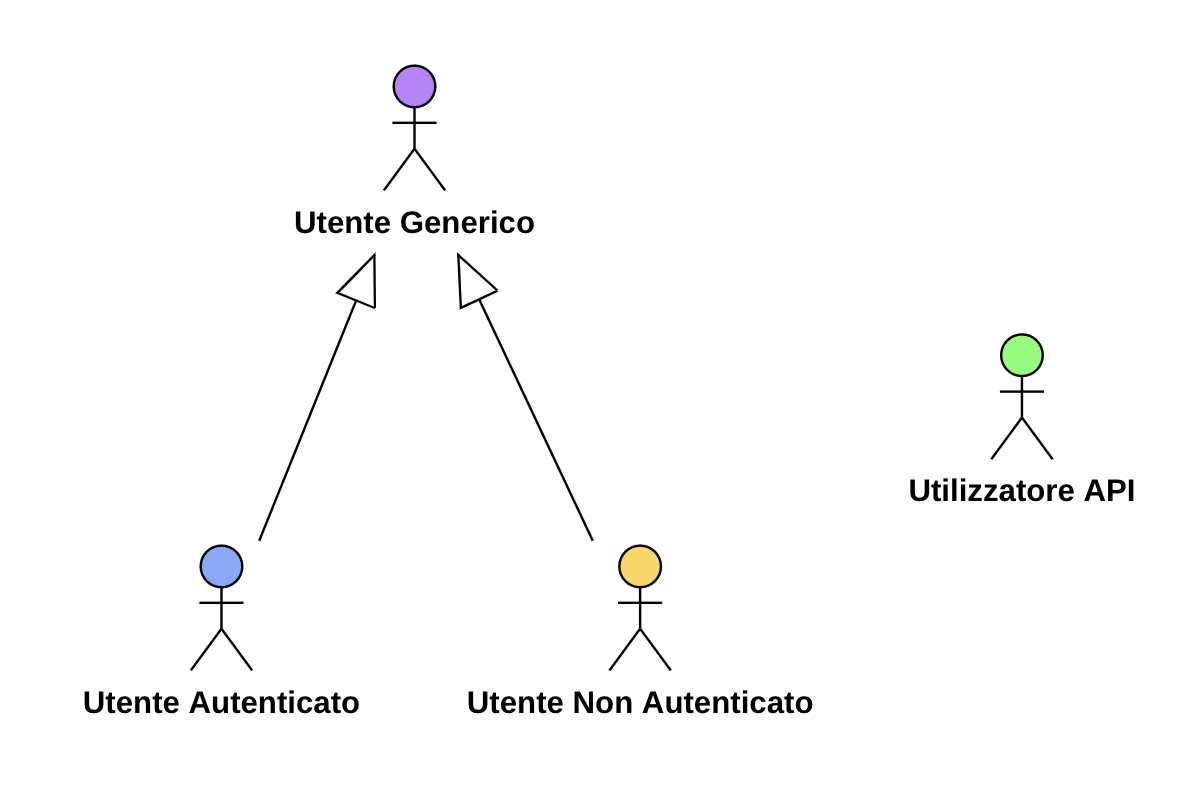
\includegraphics[scale=0.4]{src/img/attori_primari.png}
                \caption{Gerarchia degli attori primari}
            \end{figure}

            \paragraph*{Utente generico:} utente che non possiede un account \textit{MetaMask} e ha dunque possibilità di usufruire del servizio solo in lettura.

            \paragraph*{Utente non autenticato:} utente che possiede un account \textit{MetaMask} ma non è autenticato, dunque può usufruire del servizio solo in lettura o autenticarsi per poter effettuare pagamenti e rilasciare recensioni.

            \paragraph*{Utente autenticato:} utente che possiede un account \textit{MetaMask} e che è autenticato, dunque può effettuare pagamenti e rilasciare recensioni.

            \paragraph*{Utilizzatore API:} utente autenticato che utilizza l'API REST per ottenere le recensioni associate ad un utente in formato \textit{JSON}\glo, senza passare per la \textit{web app}.

        \subsubsection{Attori secondari}
            \paragraph*{\textit{MetaMask}:} \textit{wallet}\glo\: di criptovalute usato per interagire con la \textit{blockchain} \textit{Ethereum}. Permette di accedere al proprio \textit{wallet} attraverso applicazione mobile o, come nel nostro caso, estensione per browser.

            \paragraph*{\textit{Infura}\glo:} backend \textit{Web3}\glo\: che offre servizi e strumenti per sviluppatori \textit{blockchain}; nel nostro caso sarà ciò che metterà in comunicazione \textit{web app} e \textit{API REST} con nodi\glo\: sulla \textit{blockchain}.

    \subsection{Elenco}

        \subsubsection{UC01 - Autenticazione}
        \label{UC01}

            \begin{figure}[H]
                \centering
                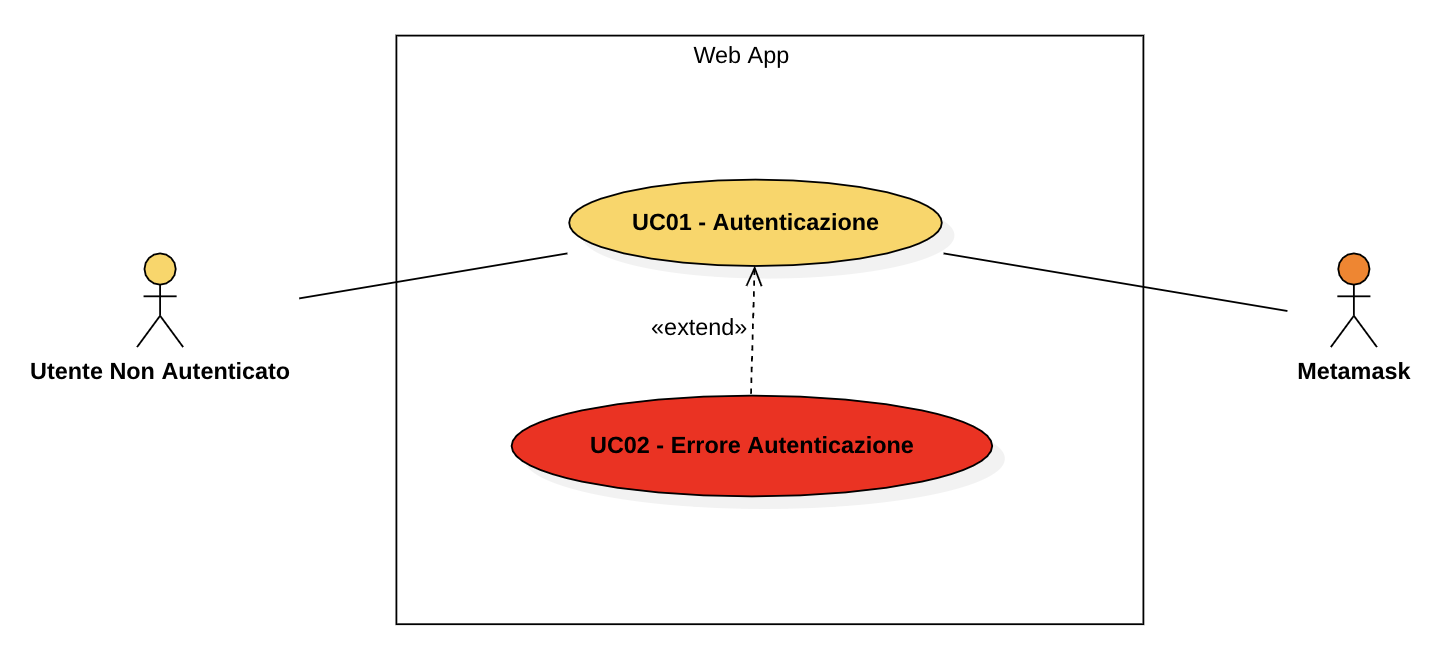
\includegraphics[scale=0.6]{src/img/UC01.png}
                \caption{UC01}
            \end{figure}

            \begin{table}[H]
                \centering
                \rowcolors{1}{pari_alt}{dispari_alt}
                \renewcommand{\arraystretch}{1.8}
                \renewcommand\tabularxcolumn[1]{m{#1}}
                \begin{tabularx}{0.9\textwidth} {
                    >{\hsize=.8\hsize\linewidth=\hsize}X
                    >{\hsize=1.2\hsize\linewidth=\hsize}X}
                    \hline
                    \textbf{Attore primario} & Utente non autenticato \\
                    \hline
                    \textbf{Attore secondario} & \textit{MetaMask} \\
                    \hline
                    \textbf{Precondizioni} & L'utente non è autenticato. \\
                    \hline
                    \textbf{Postcondizioni} & L'utente è autenticato. \\
                    \hline
                    \textbf{Scenario principale} & L'utente accede a \textit{MetaMask}. \\
                    \hline
                    \textbf{Estensioni} & Se l'accesso a \textit{MetaMask} non va a buon fine, si verifica \hyperref[UC02]{UC02}. \\
                    \hline
                \end{tabularx}
                \caption{UC01}
            \end{table}

            \subsubsection{UC02 - Errore Autenticazione}
            \label{UC02}
    
                \begin{table}[H]
                    \centering
                    \rowcolors{1}{pari_alt}{dispari_alt}
                    \renewcommand{\arraystretch}{1.8}
                    \renewcommand\tabularxcolumn[1]{m{#1}}
                    \begin{tabularx}{0.9\textwidth} {
                        >{\hsize=.8\hsize\linewidth=\hsize}X
                        >{\hsize=1.2\hsize\linewidth=\hsize}X}
                        \hline
                        \textbf{Attore primario} & Utente non autenticato \\
                        \hline
                        \textbf{Attore secondario} & \textit{MetaMask} \\
                        \hline
                        \textbf{Precondizioni} & L'utente sta tentando di autenticarsi. \\
                        \hline
                        \textbf{Postcondizioni} & L'operazione fallisce. \\
                        \hline
                        \textbf{Scenario principale} &
                            \begin{enumerate}
                                \item Si verificano problemi con l'accesso a \textit{MetaMask};
                                \item Viene mostrato un errore che informa l'utente del fallimento dell'operazione;
                                \item Vengono mostrati dei consigli sulla risoluzione del problema e si invita
                                l'utente a riprovare.
                            \end{enumerate} \\
                        \hline
                    \end{tabularx}
                    \caption{UC02}
                \end{table}

        \subsubsection{UC03 - Logout}
        \label{UC03}

            \begin{figure}[H]
                \centering
                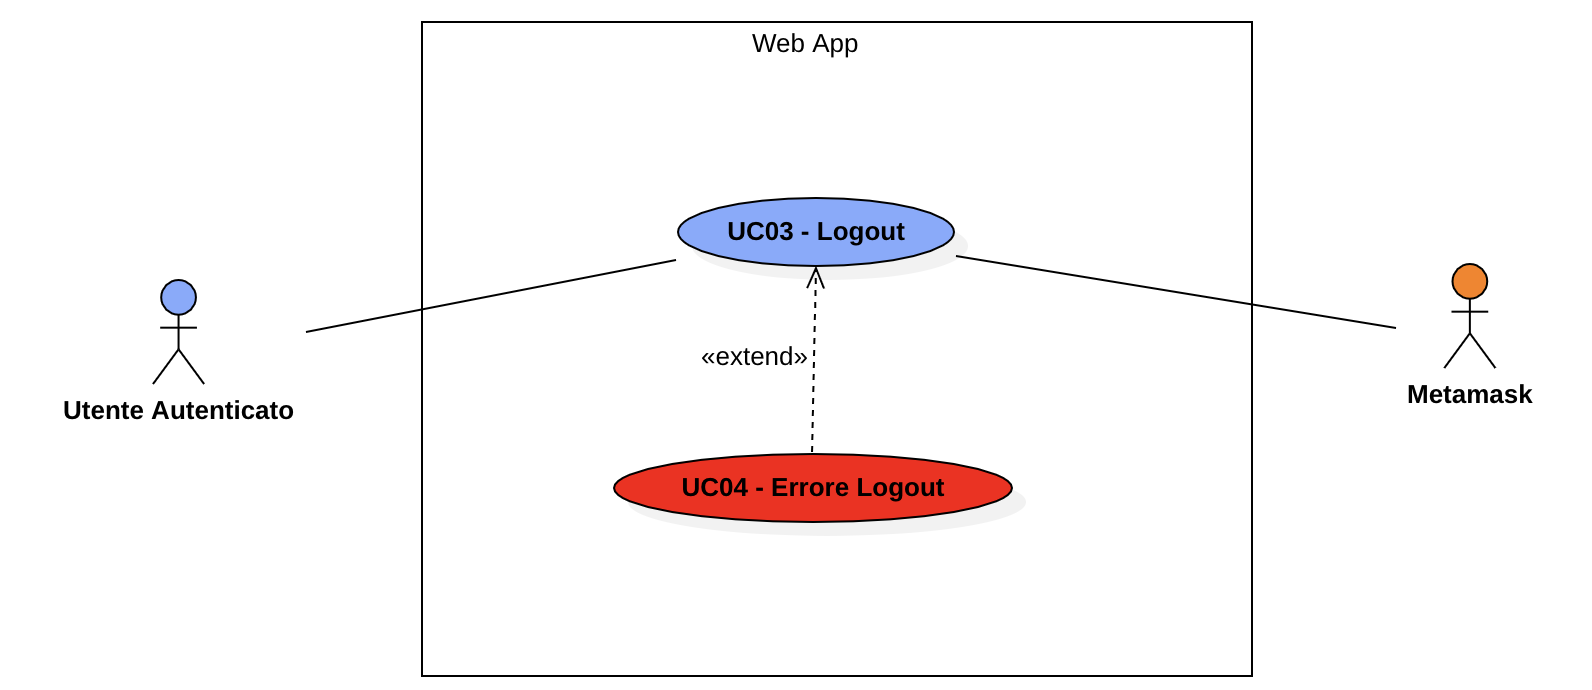
\includegraphics[scale=0.6]{src/img/UC03.png}
                \caption{UC03}
            \end{figure}

            \begin{table}[H]
                \centering
                \rowcolors{1}{pari_alt}{dispari_alt}
                \renewcommand{\arraystretch}{1.8}
                \renewcommand\tabularxcolumn[1]{m{#1}}
                \begin{tabularx}{0.9\textwidth} {
                    >{\hsize=.8\hsize\linewidth=\hsize}X
                    >{\hsize=1.2\hsize\linewidth=\hsize}X}
                    \hline
                    \textbf{Attore primario} & Utente autenticato \\
                    \hline
                    \textbf{Precondizioni} & L'utente è autenticato. \\
                    \hline
                    \textbf{Postcondizioni} & L'utente non è più autenticato. \\
                    \hline
                    \textbf{Scenario principale} & L'utente effettua il logout. \\
                    \hline
                    \textbf{Estensioni} & Se l'operazione non va a buon fine, si verifica \hyperref[UC04]{UC04}. \\
                \end{tabularx}
                \caption{UC03}
            \end{table}

            \subsubsection{UC04 - Errore Logout}
            \label{UC04}
    
                \begin{table}[H]
                    \centering
                    \rowcolors{1}{pari_alt}{dispari_alt}
                    \renewcommand{\arraystretch}{1.8}
                    \renewcommand\tabularxcolumn[1]{m{#1}}
                    \begin{tabularx}{0.9\textwidth} {
                        >{\hsize=.8\hsize\linewidth=\hsize}X
                        >{\hsize=1.2\hsize\linewidth=\hsize}X}
                        \hline
                        \textbf{Attore primario} & Utente autenticato \\
                        \hline
                        \textbf{Attore secondario} & \textit{MetaMask} \\
                        \hline
                        \textbf{Precondizioni} & L'utente sta tentando di effettuare il logout. \\
                        \hline
                        \textbf{Postcondizioni} & L'operazione fallisce. \\
                        \hline
                        \textbf{Scenario principale} &
                            \begin{enumerate}
                                \item Si verificano problemi con il logout da \textit{MetaMask};
                                \item Viene mostrato un errore che informa l'utente del fallimento dell'operazione;
                                \item Vengono mostrati dei consigli sulla risoluzione del problema e si invita
                                l'utente a riprovare.
                            \end{enumerate} \\
                        \hline
                    \end{tabularx}
                    \caption{UC04}
                \end{table}

            \subsubsection{UC05 - Transazione}
            \label{UC05}
    
                \begin{figure}[H]
                    \centering
                    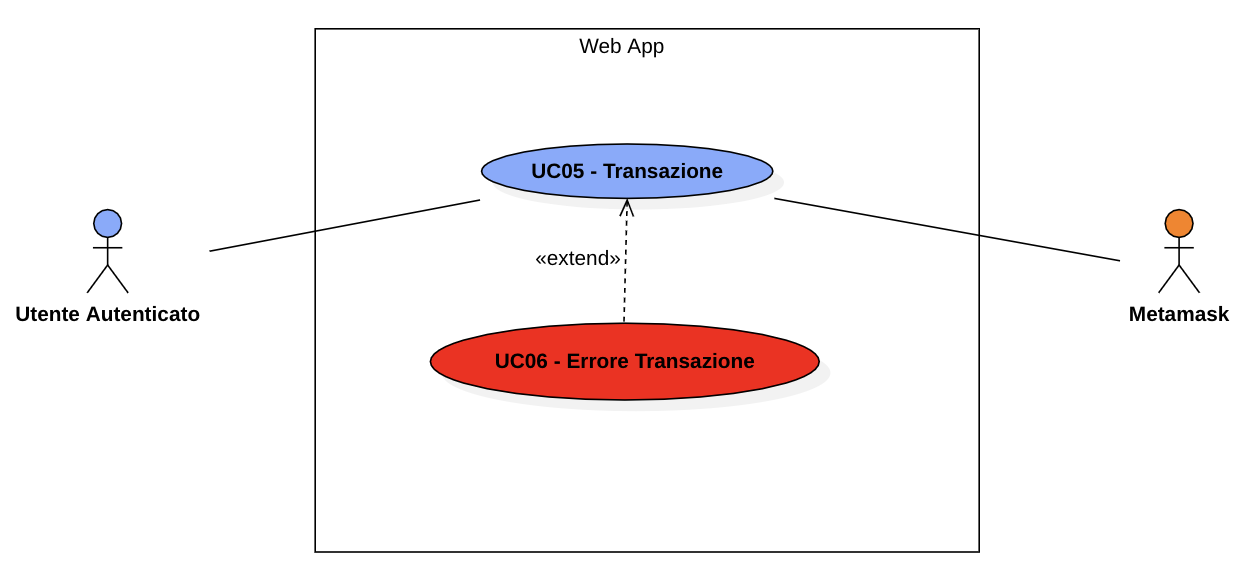
\includegraphics[scale=0.6]{src/img/UC05.png}
                    \caption{UC05}
                \end{figure}
    
                \begin{table}[H]
                    \centering
                    \rowcolors{1}{pari_alt}{dispari_alt}
                    \renewcommand{\arraystretch}{1.8}
                    \renewcommand\tabularxcolumn[1]{m{#1}}
                    \begin{tabularx}{0.9\textwidth} {
                        >{\hsize=.8\hsize\linewidth=\hsize}X
                        >{\hsize=1.2\hsize\linewidth=\hsize}X}
                        \hline
                        \textbf{Attore primario} & Utente autenticato \\
                        \hline
                        \textbf{Attore secondario} & \textit{MetaMask} \\
                        \hline
                        \textbf{Precondizioni} & L'utente non ha ancora pagato. \\
                        \hline
                        \textbf{Postcondizioni} & L'utente ha completato il pagamento. \\
                        \hline
                        \textbf{Scenario principale} & L'utente effettua il pagamento verso un altro utente. \\
                        \hline
                        \textbf{Estensioni} & Se l'operazione non va a buone fine, si verifica \hyperref[UC06]{UC06}.\\
                        \hline
                    \end{tabularx}
                    \caption{UC05}
                \end{table}

            \subsubsection{UC06 - Errore Transazione}
            \label{UC06}
    
                \begin{table}[H]
                    \centering
                    \rowcolors{1}{pari_alt}{dispari_alt}
                    \renewcommand{\arraystretch}{1.8}
                    \renewcommand\tabularxcolumn[1]{m{#1}}
                    \begin{tabularx}{0.9\textwidth} {
                        >{\hsize=.8\hsize\linewidth=\hsize}X
                        >{\hsize=1.2\hsize\linewidth=\hsize}X}
                        \hline
                        \textbf{Attore primario} & Utente autenticato \\
                        \hline
                        \textbf{Attore secondario} & \textit{MetaMask} \\
                        \hline
                        \textbf{Precondizioni} & L'utente sta tentando di effettuare un pagamento. \\
                        \hline
                        \textbf{Postcondizioni} & Il pagamento fallisce. \\
                        \hline
                        \textbf{Scenario principale} &
                        \begin{enumerate}
                            \item L'utente tenta di effettuare un pagamento che non va a buon fine;
                            \item viene mostrato un errore che informa l'utente sul motivo del fallimento dell'operazione:
                            \begin{itemize}
                                \item l'utente pagante non ha abbastanza fondi;
                                \item indirizzo dell'utente ricevente inesistente;
                            \end{itemize}
                            \item l'operazione viene annullata.
                        \end{enumerate} \\
                        \hline
                    \end{tabularx}
                    \caption{UC06}
                \end{table}

        \subsubsection{UC07 - Rilascio Recensione}
        \label{UC08}

            \begin{figure}[H]
                \centering
                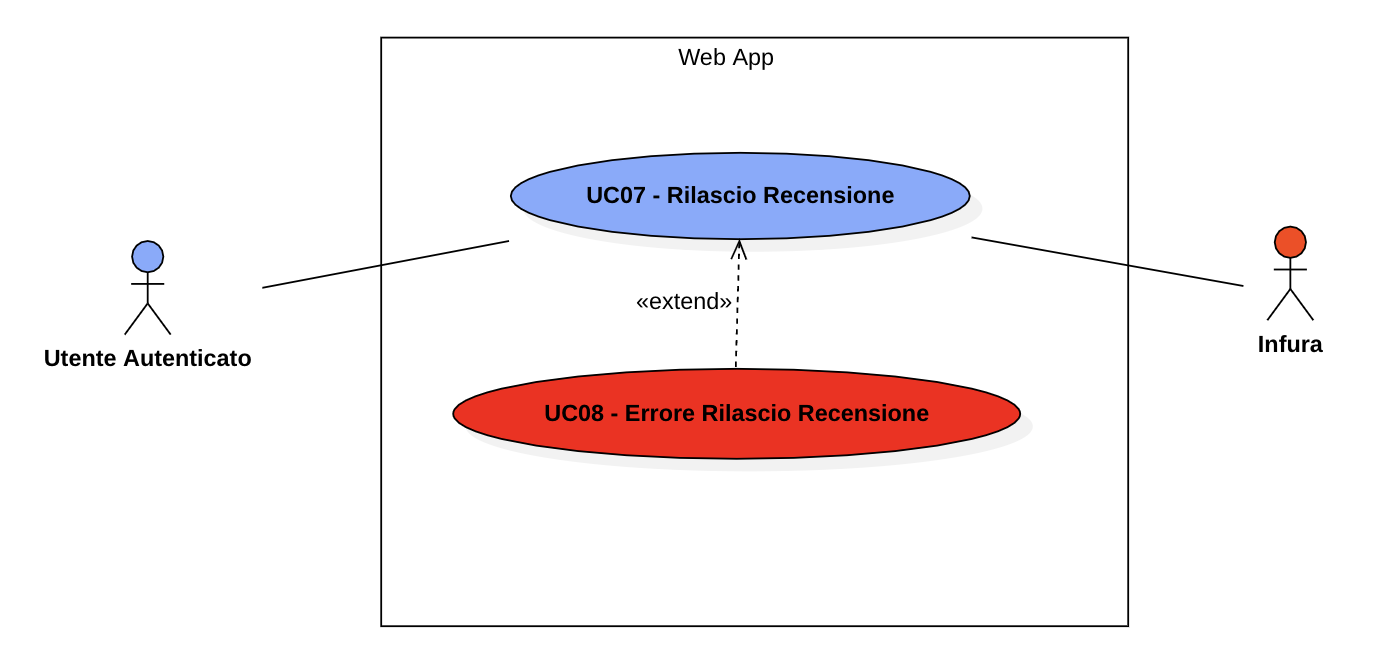
\includegraphics[scale=0.6]{src/img/UC07.png}
                \caption{UC07}
            \end{figure}

            \begin{table}[H]
                \centering
                \rowcolors{1}{pari_alt}{dispari_alt}
                \renewcommand{\arraystretch}{1.8}
                \renewcommand\tabularxcolumn[1]{m{#1}}
                \begin{tabularx}{0.9\textwidth}{
                    >{\hsize=.8\hsize\linewidth=\hsize}X
                    >{\hsize=1.2\hsize\linewidth=\hsize}X}
                    \hline
                    \textbf{Attore primario} & Utente autenticato \\
                    \hline
                    \textbf{Attore secondario} & \textit{Infura} \\
                    \hline
                    \textbf{Precondizioni} &
                        \begin{itemize}
                            \item L'utente è autenticato;
                            \item l'utente ha effettuato almeno un acquisto;
                            \item l'utente ha acquisti non recensiti.
                        \end{itemize} \\
                    \hline
                    \textbf{Postcondizioni} & L'utente ha effettuato una recensione sull'acquisto. \\
                    \hline
                    \textbf{Scenario principale} &
                        \begin{enumerate}
                            \item L'utente seleziona un pagamento da associare alla recensione;
                            \item l'utente inserisce la recensione.
                        \end{enumerate} \\
                    \hline
                    \textbf{Estensioni} & Se l'utente seleziona una pagamento già recensito, si verifica \hyperref[UC08]{UC08}. \\
                    \hline
                \end{tabularx}
                \caption{UC07}
            \end{table}

        \subsubsection{UC08 - Errore Rilascio Recensione}
        \label{UC08}

            \begin{table}[H]
                \centering
                \rowcolors{1}{pari_alt}{dispari_alt}
                \renewcommand{\arraystretch}{1.8}
                \renewcommand\tabularxcolumn[1]{m{#1}}
                \begin{tabularx}{0.9\textwidth} {
                    >{\hsize=.8\hsize\linewidth=\hsize}X
                    >{\hsize=1.2\hsize\linewidth=\hsize}X}
                    \hline
                    \textbf{Attore primario} & Utente autenticato \\
                    \hline
                    \textbf{Attore secondario} & \textit{MetaMask} \\
                    \hline
                    \textbf{Precondizioni} & L'utente vuole rilasciare una recensione. \\
                    \hline
                    \textbf{Postcondizioni} & L'operazione fallisce. \\
                    \hline
                    \textbf{Scenario principale} &
                        \begin{enumerate}
                            \item L'utente inserisce una recensione che non può rilasciare:
                            \begin{itemize}
                            \item non ha un acquisto valido legato al prodotto o servizio che vuole recensire;
                            \item la recensione non rispetta un formato valido.
                            \end{itemize}
                            \item Viene mostrato un errore che informa l'utente sulla motivazione;
                            \item vengono mostrati dei consigli sulla risoluzione del problema e si blocca
                            l'attuale operazione.
                        \end{enumerate} \\
                    \hline
                \end{tabularx}
                \caption{UC08}
            \end{table}

        \subsubsection{UC09 - Ricerca Recensioni}
        \label{UC09}

            \begin{figure}[H]
                \centering
                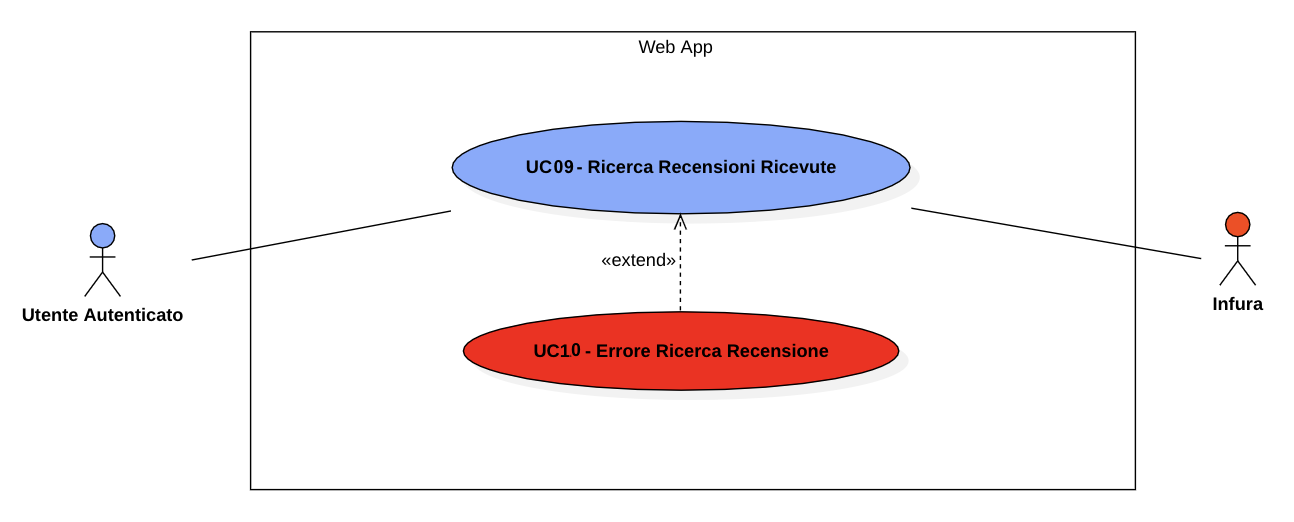
\includegraphics[scale=0.6]{src/img/UC09.png}
                \caption{UC09}
            \end{figure}

            \begin{table}[H]
                \centering
                \rowcolors{1}{pari_alt}{dispari_alt}
                \renewcommand{\arraystretch}{1.8}
                \renewcommand\tabularxcolumn[1]{m{#1}}
                \begin{tabularx}{0.9\textwidth} {
                    >{\hsize=.8\hsize\linewidth=\hsize}X
                    >{\hsize=1.2\hsize\linewidth=\hsize}X}
                    \hline
                    \textbf{Attore primario} & Utente generico \\
                    \hline
                    \textbf{Attore secondario} & Infura \\
                    \hline
                    \textbf{Precondizioni} & L'utente vuole ricercare delle recensioni. \\
                    \hline
                    \textbf{Postcondizioni} & L'utente ha ricercato delle recensioni. \\
                    \hline
                    \textbf{Scenario principale} & L'utente ricerca delle recensioni \\
                    \hline
                    \textbf{Estensioni} & Se l'operazione non va a buon fine, si verifica \hyperref[UC12]{UC12}. \\
                    \hline
                \end{tabularx}
                \caption{UC09}
            \end{table}

        \subsubsection{UC09.1 - Ricerca Recensioni per indirizzo}
        \label{UC09.1}

            \begin{figure}[H]
                \centering
                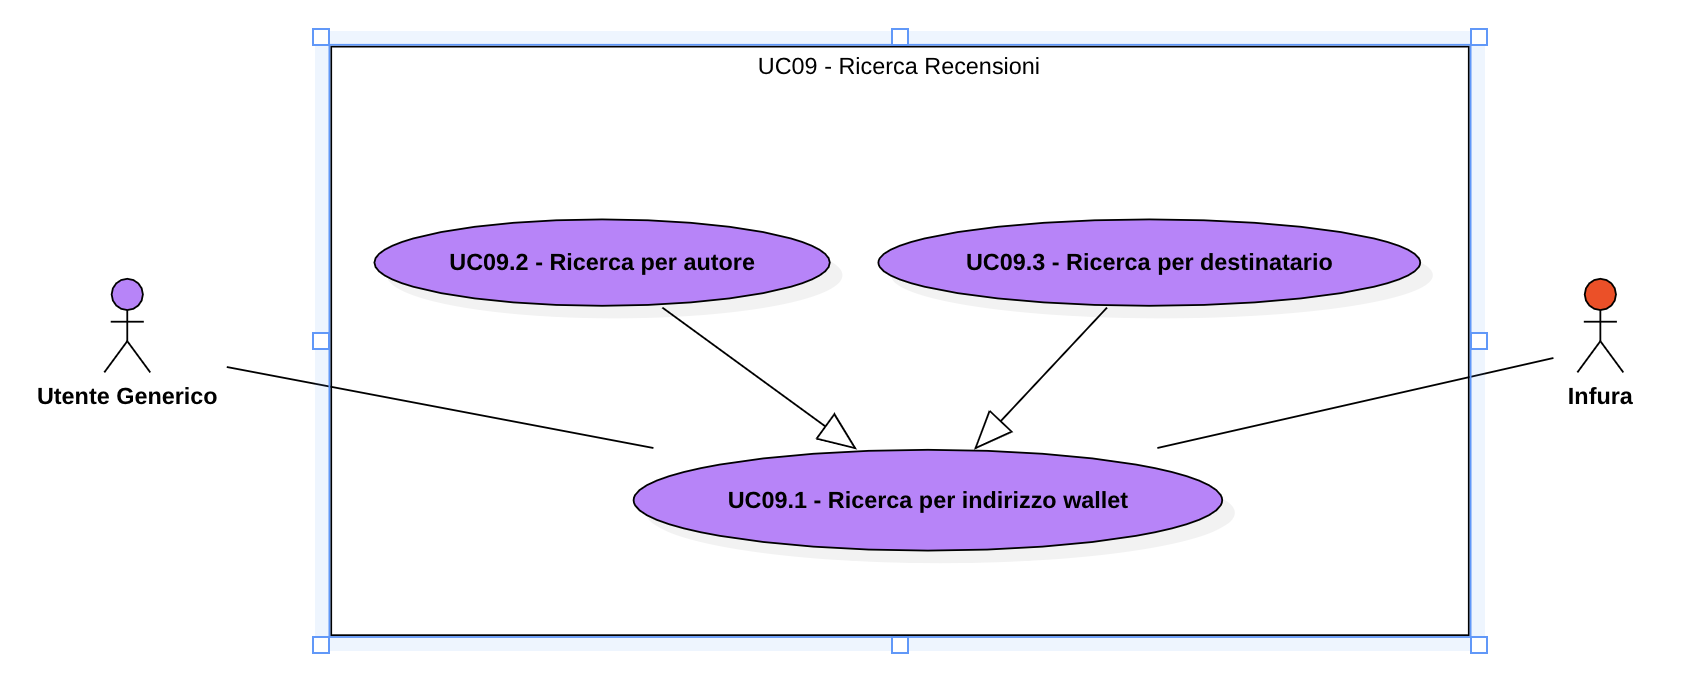
\includegraphics[scale=0.6]{src/img/UC09.1.png}
                \caption{UC09.1}
            \end{figure}

            \begin{table}[H]
                \centering
                \rowcolors{1}{pari_alt}{dispari_alt}
                \renewcommand{\arraystretch}{1.8}
                \renewcommand\tabularxcolumn[1]{m{#1}}
                \begin{tabularx}{0.9\textwidth} {
                    >{\hsize=.8\hsize\linewidth=\hsize}X
                    >{\hsize=1.2\hsize\linewidth=\hsize}X}
                    \hline
                    \textbf{Attore primario} & Utente generico \\
                    \hline
                    \textbf{Attore secondario} & Infura \\
                    \hline
                    \textbf{Precondizioni} & L'utente vuole ricercare delle recensioni legate ad un indirizzo wallet. \\
                    \hline
                    \textbf{Postcondizioni} & L'utente ha ricercato delle recensioni legate ad un indirizzo wallet. \\
                    \hline
                    \textbf{Scenario principale} & L'utente ricerca delle recensioni legate ad un indirizzo wallet.\\
                    \hline
                    \textbf{Estensioni} & Se l'operazione non va a buon fine, si verifica \hyperref[UC12]{UC12}. \\
                    \hline
                \end{tabularx}
                \caption{UC09.1}
            \end{table}

        \subsubsection{UC09.2 - Ricerca Recensioni per autore}
        \label{UC09.2}

            \begin{table}[H]
                \centering
                \rowcolors{1}{pari_alt}{dispari_alt}
                \renewcommand{\arraystretch}{1.8}
                \renewcommand\tabularxcolumn[1]{m{#1}}
                \begin{tabularx}{0.9\textwidth} {
                    >{\hsize=.8\hsize\linewidth=\hsize}X
                    >{\hsize=1.2\hsize\linewidth=\hsize}X}
                    \hline
                    \textbf{Attore primario} & Utente generico \\
                    \hline
                    \textbf{Attore secondario} & Infura \\
                    \hline
                    \textbf{Precondizioni} & L'utente vuole ricercare delle recensioni legate ad un indirizzo wallet dell'autore. \\
                    \hline
                    \textbf{Postcondizioni} & L'utente ha ricercato delle recensioni legate ad un indirizzo wallet dell'autore. \\
                    \hline
                    \textbf{Scenario principale} & L'utente ricerca delle recensioni legate ad un indirizzo wallet dell'autore.\\
                    \hline
                    \textbf{Estensioni} & Se l'operazione non va a buon fine, si verifica \hyperref[UC12]{UC12}. \\
                    \hline
                \end{tabularx}
                \caption{UC09.2}
            \end{table}

        \subsubsection{UC09.3 - Ricerca Recensioni per destinatario}
        \label{UC09.3}

            \begin{table}[H]
                \centering
                \rowcolors{1}{pari_alt}{dispari_alt}
                \renewcommand{\arraystretch}{1.8}
                \renewcommand\tabularxcolumn[1]{m{#1}}
                \begin{tabularx}{0.9\textwidth} {
                    >{\hsize=.8\hsize\linewidth=\hsize}X
                    >{\hsize=1.2\hsize\linewidth=\hsize}X}
                    \hline
                    \textbf{Attore primario} & Utente generico \\
                    \hline
                    \textbf{Attore secondario} & Infura \\
                    \hline
                    \textbf{Precondizioni} & L'utente vuole ricercare delle recensioni legate ad un indirizzo wallet del destinatario. \\
                    \hline
                    \textbf{Postcondizioni} & L'utente ha ricercato delle recensioni legate ad un indirizzo wallet del destinatario. \\
                    \hline
                    \textbf{Scenario principale} & L'utente ricerca delle recensioni legate ad un indirizzo wallet del destinatario.\\
                    \hline
                    \textbf{Estensioni} & Se l'operazione non va a buon fine, si verifica \hyperref[UC12]{UC12}. \\
                    \hline
                \end{tabularx}
                \caption{UC09.3}
            \end{table}

        \subsubsection{UC09.4 - Ricerca Recensioni per voto}
        \label{UC09.4}

            \begin{figure}[H]
                \centering
                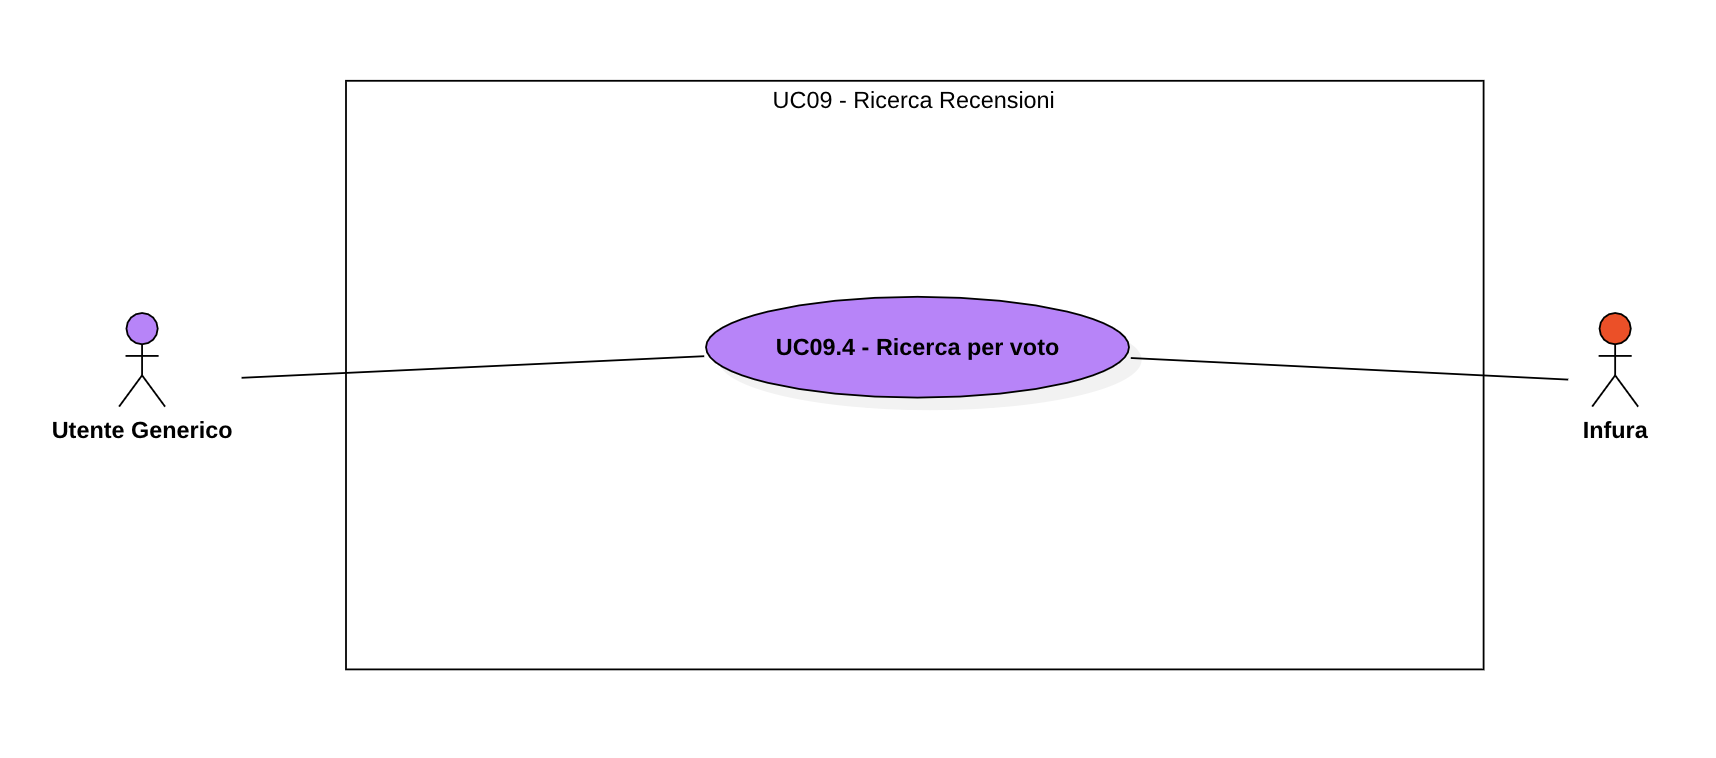
\includegraphics[scale=0.6]{src/img/UC09.4.png}
                \caption{UC09.4}
            \end{figure}

            \begin{table}[H]
                \centering
                \rowcolors{1}{pari_alt}{dispari_alt}
                \renewcommand{\arraystretch}{1.8}
                \renewcommand\tabularxcolumn[1]{m{#1}}
                \begin{tabularx}{0.9\textwidth} {
                    >{\hsize=.8\hsize\linewidth=\hsize}X
                    >{\hsize=1.2\hsize\linewidth=\hsize}X}
                    \hline
                    \textbf{Attore primario} & Utente generico \\
                    \hline
                    \textbf{Attore secondario} & Infura \\
                    \hline
                    \textbf{Precondizioni} & L'utente vuole ricercare delle recensioni per votazione. \\
                    \hline
                    \textbf{Postcondizioni} & L'utente ha ricercato delle recensioni votazione. \\
                    \hline
                    \textbf{Scenario principale} & L'utente ricerca delle recensioni per votazione.\\
                    \hline
                    \textbf{Estensioni} & Se l'operazione non va a buon fine, si verifica \hyperref[UC12]{UC12}. \\
                    \hline
                \end{tabularx}
                \caption{UC09.4}
            \end{table}

        \subsubsection{UC09.5 - Ricerca Recensioni per titolo}
        \label{UC09.5}

            \begin{figure}[H]
                \centering
                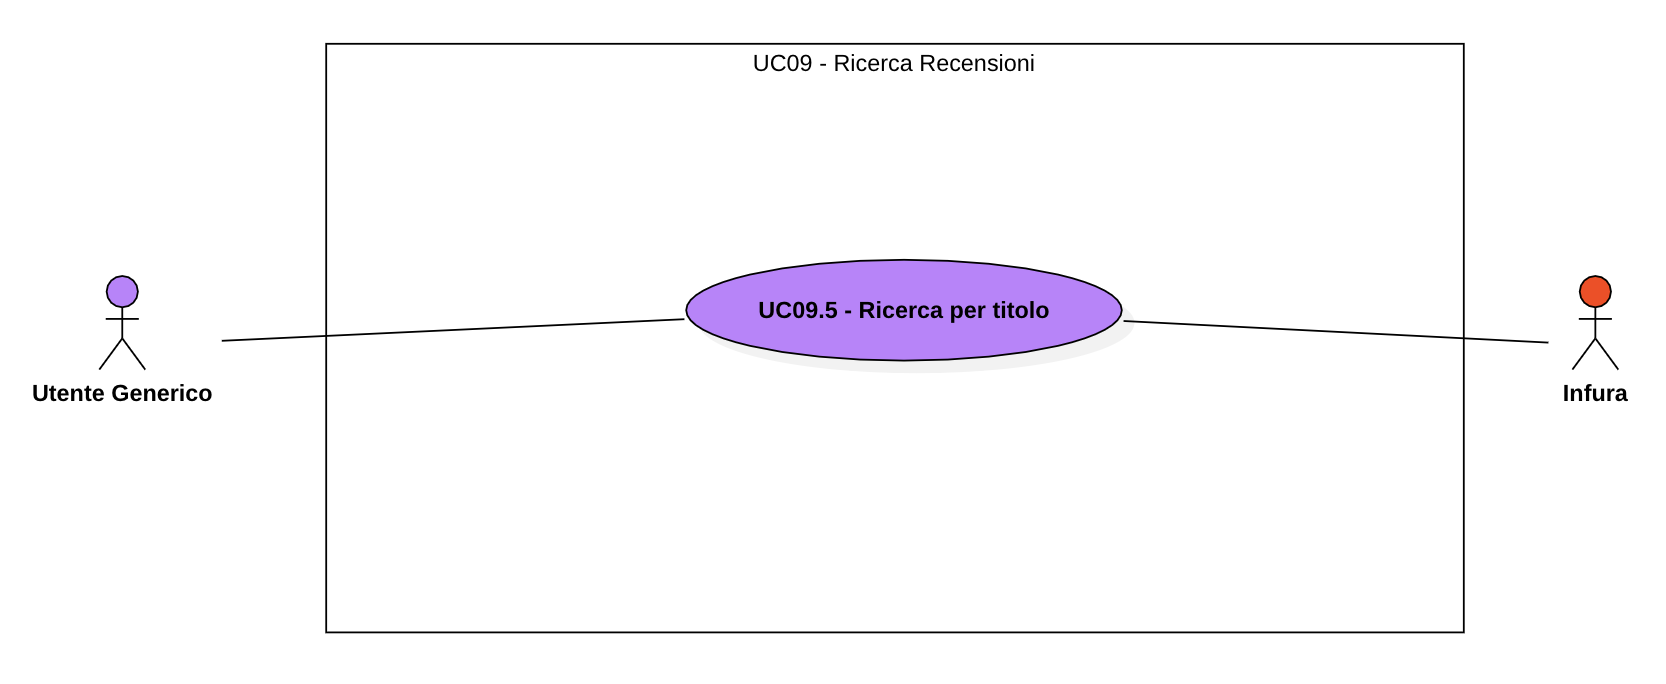
\includegraphics[scale=0.6]{src/img/UC09.5.png}
                \caption{UC09.5}
            \end{figure}

            \begin{table}[H]
                \centering
                \rowcolors{1}{pari_alt}{dispari_alt}
                \renewcommand{\arraystretch}{1.8}
                \renewcommand\tabularxcolumn[1]{m{#1}}
                \begin{tabularx}{0.9\textwidth} {
                    >{\hsize=.8\hsize\linewidth=\hsize}X
                    >{\hsize=1.2\hsize\linewidth=\hsize}X}
                    \hline
                    \textbf{Attore primario} & Utente generico \\
                    \hline
                    \textbf{Attore secondario} & Infura \\
                    \hline
                    \textbf{Precondizioni} & L'utente vuole ricercare delle recensioni legate ad un titolo, ovvero nome del prodotto o servizio acquistato. \\
                    \hline
                    \textbf{Postcondizioni} & L'utente ha ricercato delle recensioni legate ad un titolo, ovvero nome del prodotto o servizio acquistato. \\
                    \hline
                    \textbf{Scenario principale} & L'utente ricerca delle recensioni legate ad un titolo, ovvero nome del prodotto o servizio acquistato.\\
                    \hline
                    \textbf{Estensioni} & Se l'operazione non va a buon fine, si verifica \hyperref[UC12]{UC12}. \\
                    \hline
                \end{tabularx}
                \caption{UC09.5}
            \end{table}

        \subsubsection{UC09.6 - Ricerca Recensioni per data}
        \label{UC09.6}

            \begin{figure}[H]
                \centering
                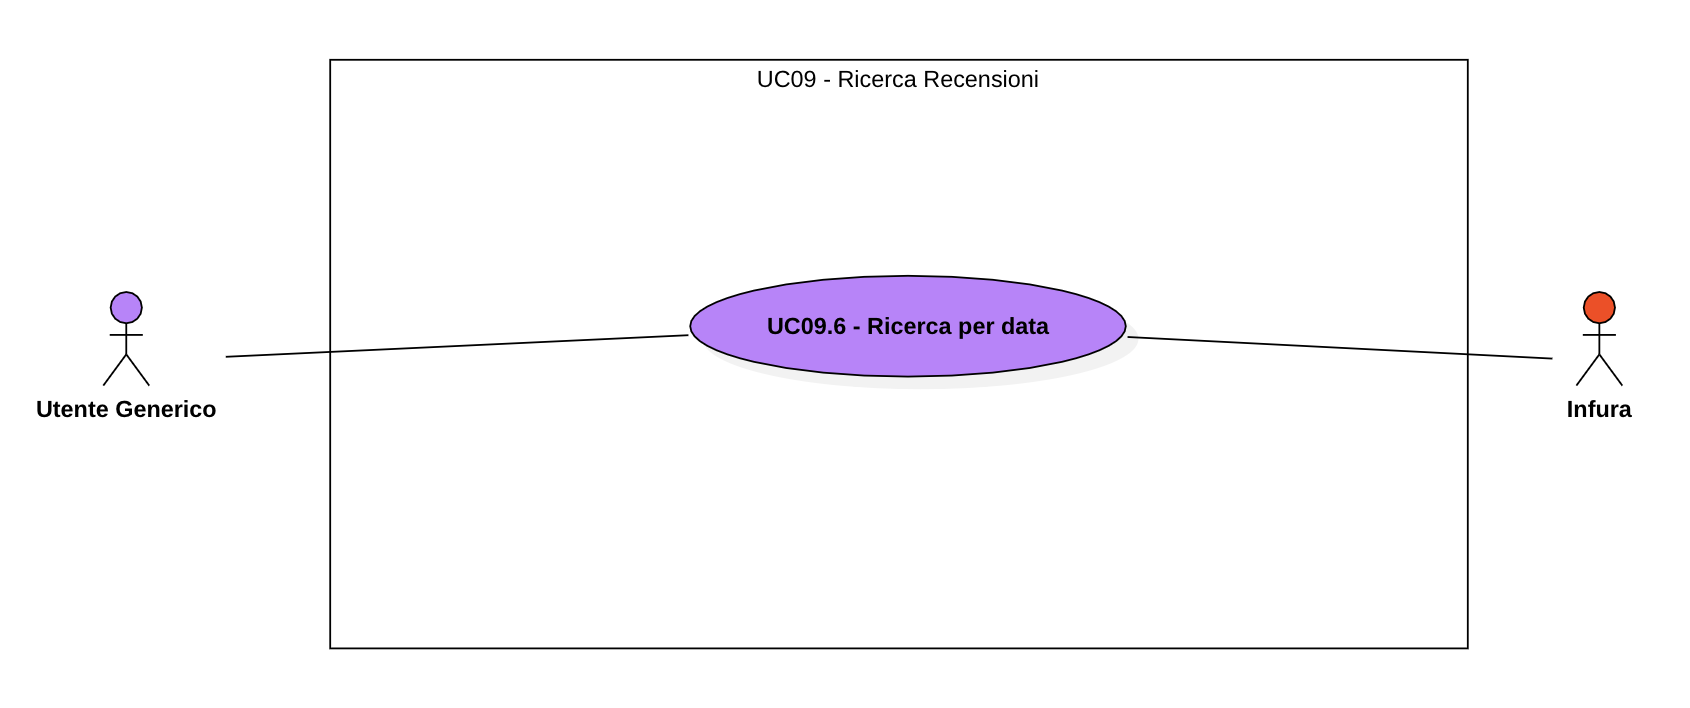
\includegraphics[scale=0.6]{src/img/UC09.6.png}
                \caption{UC09.6}
            \end{figure}

            \begin{table}[H]
                \centering
                \rowcolors{1}{pari_alt}{dispari_alt}
                \renewcommand{\arraystretch}{1.8}
                \renewcommand\tabularxcolumn[1]{m{#1}}
                \begin{tabularx}{0.9\textwidth} {
                    >{\hsize=.8\hsize\linewidth=\hsize}X
                    >{\hsize=1.2\hsize\linewidth=\hsize}X}
                    \hline
                    \textbf{Attore primario} & Utente generico \\
                    \hline
                    \textbf{Attore secondario} & Infura \\
                    \hline
                    \textbf{Precondizioni} & L'utente vuole ricercare delle recensioni per data di pubblicazione. \\
                    \hline
                    \textbf{Postcondizioni} & L'utente ha ricercato delle recensioni per data di pubblicazione. \\
                    \hline
                    \textbf{Scenario principale} & L'utente ricerca delle recensioni per data di pubblicazione.\\
                    \hline
                    \textbf{Estensioni} & Se l'operazione non va a buon fine, si verifica \hyperref[UC12]{UC12}. \\
                    \hline
                \end{tabularx}
                \caption{UC09.6}
            \end{table}

        \subsubsection{UC12 - Errore Ricerca Recensioni}
        \label{UC12}

            \begin{table}[H]
                \centering
                \rowcolors{1}{pari_alt}{dispari_alt}
                \renewcommand{\arraystretch}{1.8}
                \renewcommand\tabularxcolumn[1]{m{#1}}
                \begin{tabularx}{0.9\textwidth} {
                    >{\hsize=.8\hsize\linewidth=\hsize}X
                    >{\hsize=1.2\hsize\linewidth=\hsize}X}
                    \hline
                    \textbf{Attori primari} & Utente generico, utente autenticato. \\
                    \hline
                    \textbf{Attore secondario} & \textit{Infura} \\
                    \hline
                    \textbf{Precondizioni} & L'utente richiede le recensioni collegate ad un indirizzo. \\
                    \hline
                    \textbf{Postcondizioni} & La ricerca fallisce. \\
                    \hline
                    \textbf{Scenario principale} & L'utente inserisce un indirizzo inesistente e viene visualizzato un errore. \\
                    \hline
                \end{tabularx}
                \caption{UC12}
            \end{table}

        \subsubsection{UC0Y - Visualizzazione Recensioni}
        \label{UC0Y}

            \begin{figure}[H]
                \centering
                \includesvg[width=1\textwidth]{src/img/UC04.drawio.svg}
                \caption{UC04}
            \end{figure}

            \begin{table}[H]
                \centering
                \rowcolors{1}{pari_alt}{dispari_alt}
                \renewcommand{\arraystretch}{1.8}
                \renewcommand\tabularxcolumn[1]{m{#1}}
                \begin{tabularx}{0.9\textwidth} {
                    >{\hsize=.8\hsize\linewidth=\hsize}X
                    >{\hsize=1.2\hsize\linewidth=\hsize}X}
                    \hline
                    \textbf{Attore primario} & Utente generico \\
                    \hline
                    \textbf{Precondizioni} & L'utente ha effettuato una ricerca per indirizzo. \\
                    \hline
                    \textbf{Postcondizioni} & L'utente visualizza le recensioni associate a quell'indirizzo. \\
                    \hline
                    \textbf{Scenario principale} & Viene visualizzata una lista di recensioni corrispondenti. \\
                    \hline
                    \textbf{Estensioni} & Se l'utente inserisce un indirizzo inesistente, si verifica \hyperref[UC12]{UC12}. \\
                    \hline
                \end{tabularx}
                \caption{UC04}
            \end{table}

        \subsubsection{UC05 - Visualizzazione Recensioni Rilasciate}
        \label{UC05}

            \begin{figure}[H]
                \centering
                \includesvg[width=1\textwidth]{src/img/UC05.drawio.svg}
                \caption{UC05}
            \end{figure}

            \begin{table}[H]
                \centering
                \rowcolors{1}{pari_alt}{dispari_alt}
                \renewcommand{\arraystretch}{1.8}
                \renewcommand\tabularxcolumn[1]{m{#1}}
                \begin{tabularx}{0.9\textwidth} {
                    >{\hsize=.8\hsize\linewidth=\hsize}X
                    >{\hsize=1.2\hsize\linewidth=\hsize}X}
                    \hline
                    \textbf{Attore primario} & Utente autenticato \\
                    \hline
                    \textbf{Attore secondario} & \textit{MetaMask} \\
                    \hline
                    \textbf{Precondizioni} & Nessuna. \\
                    \hline
                    \textbf{Postcondizioni} & L'utente visualizza le recensioni che ha rilasciato. \\
                    \hline
                    \textbf{Scenario principale} & Viene mostrata la lista di recensioni rilasciate dall'utente. \\
                    \hline
                \end{tabularx}
                \caption{UC05}
            \end{table}

        \subsubsection{UC06 - Visualizzazione Recensioni Ricevute}
        \label{UC06}

            \begin{figure}[H]
                \centering
                \includesvg[width=1\textwidth]{src/img/UC06.drawio.svg}
                \caption{UC06}
            \end{figure}

            \begin{table}[H]
                \centering
                \rowcolors{1}{pari_alt}{dispari_alt}
                \renewcommand{\arraystretch}{1.8}
                \renewcommand\tabularxcolumn[1]{m{#1}}
                \begin{tabularx}{0.9\textwidth} {
                    >{\hsize=.8\hsize\linewidth=\hsize}X
                    >{\hsize=1.2\hsize\linewidth=\hsize}X}
                    \hline
                    \textbf{Attore primario} & Utente autenticato \\
                    \hline
                    \textbf{Attore secondario} & \textit{MetaMask} \\
                    \hline
                    \textbf{Precondizioni} & Nessuna. \\
                    \hline
                    \textbf{Postcondizioni} & L'utente visualizza le recensioni che ha ricevuto. \\
                    \hline
                    \textbf{Scenario principale} & Viene mostrata la lista di recensioni ricevute dall'utente. \\
                    \hline
                \end{tabularx}
                \caption{UC06}
            \end{table}

        \subsubsection{UC07 - Visualizzazione Singola Recensione}
        \label{UC07}

            \begin{figure}[H]
                \centering
                \includesvg[width=1\textwidth]{src/img/UC07.drawio.svg}
                \caption{UC07}
            \end{figure}

            \begin{table}[H]
                \centering
                \rowcolors{1}{pari_alt}{dispari_alt}
                \renewcommand{\arraystretch}{1.8}
                \renewcommand\tabularxcolumn[1]{m{#1}}
                \begin{tabularx}{0.9\textwidth} {
                    >{\hsize=.8\hsize\linewidth=\hsize}X
                    >{\hsize=1.2\hsize\linewidth=\hsize}X}
                    \hline
                    \textbf{Attore primario} & Utente generico \\
                    \hline
                    \textbf{Precondizioni} & Si sta visualizzando una lista di recensioni. \\
                    \hline
                    \textbf{Postcondizioni} & Viene visualizzata una singola recensione della lista. \\
                    \hline
                    \textbf{Scenario principale} & Viene visualizzata una recensione appartenente alla lista richiesta dall'utente. \\
                    \hline
                \end{tabularx}
                \caption{UC07}
            \end{table}

        \subsubsection{UC07.1 - Visualizzazione Autore Recensione}
        \label{UC07.1}

            \begin{table}[H]
                \centering
                \rowcolors{1}{pari_alt}{dispari_alt}
                \renewcommand{\arraystretch}{1.8}
                \renewcommand\tabularxcolumn[1]{m{#1}}
                \begin{tabularx}{0.9\textwidth} {
                    >{\hsize=.8\hsize\linewidth=\hsize}X
                    >{\hsize=1.2\hsize\linewidth=\hsize}X}
                    \hline
                    \textbf{Attore primario} & Utente generico \\
                    \hline
                    \textbf{Precondizioni} & Viene visualizzata una recensione. \\
                    \hline
                    \textbf{Postcondizioni} & Viene visualizzato l'autore della recensione. \\
                    \hline
                    \textbf{Scenario principale} & Viene visualizzato l'autore all'interno della recensione corrispondente. \\
                    \hline
                \end{tabularx}
                \caption{UC07.1}
            \end{table}

        \subsubsection{UC07.2 - Visualizzazione Testo Recensione}
        \label{UC07.2}

            \begin{table}[H]
                \centering
                \rowcolors{1}{pari_alt}{dispari_alt}
                \renewcommand{\arraystretch}{1.8}
                \renewcommand\tabularxcolumn[1]{m{#1}}
                \begin{tabularx}{0.9\textwidth} {
                    >{\hsize=.8\hsize\linewidth=\hsize}X
                    >{\hsize=1.2\hsize\linewidth=\hsize}X}
                    \hline
                    \textbf{Attore primario} & Utente generico \\
                    \hline
                    \textbf{Precondizioni} & Viene visualizzata una recensione. \\
                    \hline
                    \textbf{Postcondizioni} & Viene visualizzato il testo della recensione. \\
                    \hline
                    \textbf{Scenario principale} & Viene visualizzato il testo all'interno della recensione corrispondente. \\
                    \hline
                \end{tabularx}
                \caption{UC7.2}
            \end{table}

        \subsubsection{UC07.3 - Visualizzazione Voto Recensione}
        \label{UC07.3}

            \begin{table}[H]
                \centering
                \rowcolors{1}{pari_alt}{dispari_alt}
                \renewcommand{\arraystretch}{1.8}
                \renewcommand\tabularxcolumn[1]{m{#1}}
                \begin{tabularx}{0.9\textwidth} {
                    >{\hsize=.8\hsize\linewidth=\hsize}X
                    >{\hsize=1.2\hsize\linewidth=\hsize}X}
                    \hline
                    \textbf{Attore primario} & Utente generico \\
                    \hline
                    \textbf{Precondizioni} & Viene visualizzata una recensione. \\
                    \hline
                    \textbf{Postcondizioni} & Viene visualizzato il voto della recensione. \\
                    \hline
                    \textbf{Scenario principale} & Viene visualizzato il voto all'interno della recensione corrispondente. \\
                    \hline
                \end{tabularx}
                \caption{UC7.3}
            \end{table}


        \subsubsection{UC09 - Pagamento}
        \label{UC09}

            \begin{figure}[H]
                \centering
                \includesvg[scale=0.9]{src/img/UC09.drawio.svg}
                \caption{UC09}
            \end{figure}

            \begin{table}[H]
                \centering
                \rowcolors{1}{pari_alt}{dispari_alt}
                \renewcommand{\arraystretch}{1.8}
                \renewcommand\tabularxcolumn[1]{m{#1}}
                \begin{tabularx}{0.9\textwidth} {
                    >{\hsize=.8\hsize\linewidth=\hsize}X
                    >{\hsize=1.2\hsize\linewidth=\hsize}X}
                    \hline
                    \textbf{Attore primario} & Utente autenticato \\
                    \hline
                    \textbf{Attore secondario} & \textit{MetaMask} \\
                    \hline
                    \textbf{Precondizioni} & L'utente non ha ancora pagato. \\
                    \hline
                    \textbf{Postcondizioni} & L'utente ha completato il pagamento. \\
                    \hline
                    \textbf{Scenario principale} & L'utente effettua il pagamento. \\
                    \hline
                    \textbf{Estensioni} & Se l'utente non ha fondi sufficienti nel \textit{wallet}, si verifica \hyperref[UC14]{UC14}.\\
                    \hline
                \end{tabularx}
                \caption{UC09}
            \end{table}

        \subsubsection{UC10 - Errore Autenticazione}
        \label{UC10}

            \begin{table}[H]
                \centering
                \rowcolors{1}{pari_alt}{dispari_alt}
                \renewcommand{\arraystretch}{1.8}
                \renewcommand\tabularxcolumn[1]{m{#1}}
                \begin{tabularx}{0.9\textwidth} {
                    >{\hsize=.8\hsize\linewidth=\hsize}X
                    >{\hsize=1.2\hsize\linewidth=\hsize}X}
                    \hline
                    \textbf{Attore primario} & Utente non autenticato \\
                    \hline
                    \textbf{Attore secondario} & \textit{MetaMask} \\
                    \hline
                    \textbf{Precondizioni} & L'utente sta tentando di autenticarsi. \\
                    \hline
                    \textbf{Postcondizioni} & L'operazione fallisce. \\
                    \hline
                    \textbf{Scenario principale} &
                        \begin{enumerate}
                            \item Si verificano problemi con l'accesso a \textit{MetaMask};
                            \item Viene mostrato un errore che informa l'utente del fallimento dell'operazione;
                            \item Vengono mostrati dei consigli sulla risoluzione del problema e si invita
                            l'utente a riprovare.
                        \end{enumerate} \\
                    \hline
                \end{tabularx}
                \caption{UC10}
            \end{table}

        \subsubsection{UC12 - Errore Visualizzazione Recensioni}
        \label{UC12}

            \begin{table}[H]
                \centering
                \rowcolors{1}{pari_alt}{dispari_alt}
                \renewcommand{\arraystretch}{1.8}
                \renewcommand\tabularxcolumn[1]{m{#1}}
                \begin{tabularx}{0.9\textwidth} {
                    >{\hsize=.8\hsize\linewidth=\hsize}X
                    >{\hsize=1.2\hsize\linewidth=\hsize}X}
                    \hline
                    \textbf{Attori primari} & Utente generico, utente autenticato. \\
                    \hline
                    \textbf{Precondizioni} & L'utente ha effettuato una ricerca per indirizzo. \\
                    \hline
                    \textbf{Postcondizioni} & L'utente non visualizza nessuna recensione. \\
                    \hline
                    \textbf{Scenario principale} &
                        \begin{enumerate}
                            \item L'utente richiede la lista delle recensioni di un determinato indirizzo;
                            \item l'indirizzo cercato non presenta recensioni collegate e l'utente viene
                            informato di questo.
                        \end{enumerate} \\
                    \hline
                \end{tabularx}
                \caption{UC12}
            \end{table}

        

        \subsubsection{UC14 - Errore Pagamento}
        \label{UC14}

            \begin{table}[H]
                \centering
                \rowcolors{1}{pari_alt}{dispari_alt}
                \renewcommand{\arraystretch}{1.8}
                \renewcommand\tabularxcolumn[1]{m{#1}}
                \begin{tabularx}{0.9\textwidth} {
                    >{\hsize=.8\hsize\linewidth=\hsize}X
                    >{\hsize=1.2\hsize\linewidth=\hsize}X}
                    \hline
                    \textbf{Attore primario} & Utente autenticato \\
                    \hline
                    \textbf{Attore secondario} & \textit{MetaMask} \\
                    \hline
                    \textbf{Precondizioni} & L'utente sta tentando di effettuare un pagamento. \\
                    \hline
                    \textbf{Postcondizioni} & Il pagamento fallisce. \\
                    \hline
                    \textbf{Scenario principale} &
                    \begin{enumerate}
                        \item L'utente tenta di effettuare un pagamento che non va a buon fine;
                        \item viene mostrato un errore che informa l'utente sul motivo del fallimento
                        dell'operazione;
                        \item l'operazione viene annullata.
                    \end{enumerate} \\
                    \hline
                \end{tabularx}
                \caption{UC14}
            \end{table}

        \subsubsection{UC15 - Richiesta Lista Recensioni}
        \label{UC15}

            \begin{figure}[H]
                \centering
                \includesvg[width=1\textwidth]{src/img/UC15.drawio.svg}
                \caption{UC15}
            \end{figure}

            \begin{table}[H]
                \centering
                \rowcolors{1}{pari_alt}{dispari_alt}
                \renewcommand{\arraystretch}{1.8}
                \renewcommand\tabularxcolumn[1]{m{#1}}
                \begin{tabularx}{0.9\textwidth} {
                    >{\hsize=.8\hsize\linewidth=\hsize}X
                    >{\hsize=1.2\hsize\linewidth=\hsize}X}
                \hline
                \textbf{Attore primario} & Utilizzatore \textit{API} \\
                \hline
                \textbf{Attore secondario} & \textit{Infura} \\
                \hline
                \textbf{Precondizioni} & L'utente conosce l'indirizzo di cui vuole visualizzare le recensioni. \\
                \hline
                \textbf{Postcondizioni} & L'utente ottiene un file contenente una lista di recensioni. \\
                \hline
                \textbf{Scenario principale} &
                    \begin{enumerate}
                        \item L'utente fa una richiesta al \textit{server API REST}\glo\: specificando l'indirizzo di cui
                        ottenere le recensioni;
                        \item il server recupera le recensioni legate all'utente richiesto;
                        \item viene restituita una lista di recensioni;
                    \end{enumerate} \\
                \hline
                \textbf{Estensioni} & Se la richiesta fallisce, si verifica \hyperref[UC16]{UC16}. \\
                \hline
                \end{tabularx}
                \caption{UC15}
            \end{table}

        \subsubsection{UC16 - Errore Ottenimento Recensioni}
        \label{UC16}

            \begin{table}[H]
                \centering
                \rowcolors{1}{pari_alt}{dispari_alt}
                \renewcommand{\arraystretch}{1.8}
                \renewcommand\tabularxcolumn[1]{m{#1}}
                \begin{tabularx}{0.9\textwidth} {
                    >{\hsize=.8\hsize\linewidth=\hsize}X
                    >{\hsize=1.2\hsize\linewidth=\hsize}X}
                    \hline
                    \textbf{Attore primario} & Utilizzatore \textit{API} \\
                    \hline
                    \textbf{Attore secondario} & \textit{Infura} \\
                    \hline
                    \textbf{Precondizioni} & L'utente sta tentando di ottenere la lista recensioni. \\
                    \hline
                    \textbf{Postcondizioni} & L'operazione fallisce. \\
                    \hline
                    \textbf{Scenario principale} &
                        \begin{enumerate}
                            \item L'utente tenta di ottenere la lista di recensioni;
                            \item viene mostrato un errore che informa l'utente sul motivo del fallimento
                            dell'operazione.
                        \end{enumerate} \\
                    \hline
                \end{tabularx}
                \caption{UC16}
            \end{table}

\pagebreak